\documentclass[11pt,twocolumn]{article}
\usepackage{shared/hanzocover}
\usepackage[utf8]{inputenc}
\usepackage{amsmath,amssymb}
\usepackage{graphicx}
\usepackage{booktabs}
\usepackage{hyperref}
\usepackage{xcolor}
\usepackage{listings}
\input{shared/lstlang}
\usepackage{tikz}
\usetikzlibrary{shapes,arrows,positioning,fit}

\definecolor{codegreen}{rgb}{0,0.6,0}
\definecolor{codegray}{rgb}{0.5,0.5,0.5}
\definecolor{codepurple}{rgb}{0.58,0,0.82}
\definecolor{backcolour}{rgb}{0.95,0.95,0.92}

\lstdefinestyle{mystyle}{
    backgroundcolor=\color{backcolour},
    commentstyle=\color{codegreen},
    keywordstyle=\color{codepurple},
    numberstyle=\tiny\color{codegray},
    stringstyle=\color{codegreen},
    basicstyle=\ttfamily\footnotesize,
    breakatwhitespace=false,
    breaklines=true,
    captionpos=b,
    keepspaces=true,
    numbers=left,
    numbersep=5pt,
    showspaces=false,
    showstringspaces=false,
    showtabs=false,
    tabsize=2
}
\lstset{style=mystyle}

\title{Hanzo Gateway: High-Performance API Gateway with JWT Validation and Rate Limiting}
\author{Zach Kelling\thanks{zach@hanzo.ai} \\ \textit{Hanzo Industries} \\ \texttt{research@hanzo.ai}}
\date{February 2019}

\begin{document}

\hanzocoverpage

\begin{abstract}
We present Hanzo Gateway, a high-performance API gateway built on the KrakenD framework that serves as the unified entry point for all Hanzo platform services. The gateway implements stateless JWT validation against Hanzo IAM, per-tenant rate limiting with sliding window counters, automatic circuit breaking for downstream failures, and request/response transformation pipelines. Processing over 147 endpoint definitions, the gateway achieves a median latency overhead of 1.2ms per request while handling 45,000 requests per second on a single node. We describe the declarative configuration model, the plugin architecture for custom middleware, and the operational patterns that enable zero-downtime configuration reloads in production.
\end{abstract}

\section{Introduction}

API gateways are a critical infrastructure component in microservice architectures, responsible for authentication, rate limiting, request routing, and protocol transformation. The gateway sits on the critical path of every API request, making performance and reliability paramount.

Hanzo Gateway extends KrakenD~\cite{krakend2017}, a stateless Go-based API gateway, with Hanzo-specific integrations: IAM JWT validation, KMS-backed configuration secrets, and Prometheus metrics aligned with the Hanzo observability stack. The stateless design is fundamental---no database, no distributed cache, no coordination between gateway instances---enabling horizontal scaling by simply adding replicas behind a load balancer.

\paragraph{Contributions.}
\begin{itemize}
    \item A declarative JSON configuration model defining 147+ endpoints with backend aggregation, response merging, and transformation rules.
    \item Stateless JWT validation using JWKS from Hanzo IAM with automatic key rotation detection.
    \item Sliding window rate limiting with per-tenant and per-endpoint granularity, implemented without external state.
    \item Circuit breaker integration with configurable thresholds, half-open probing, and automatic recovery.
\end{itemize}

\section{Architecture}

\subsection{Request Pipeline}

\begin{figure}[t]
\centering
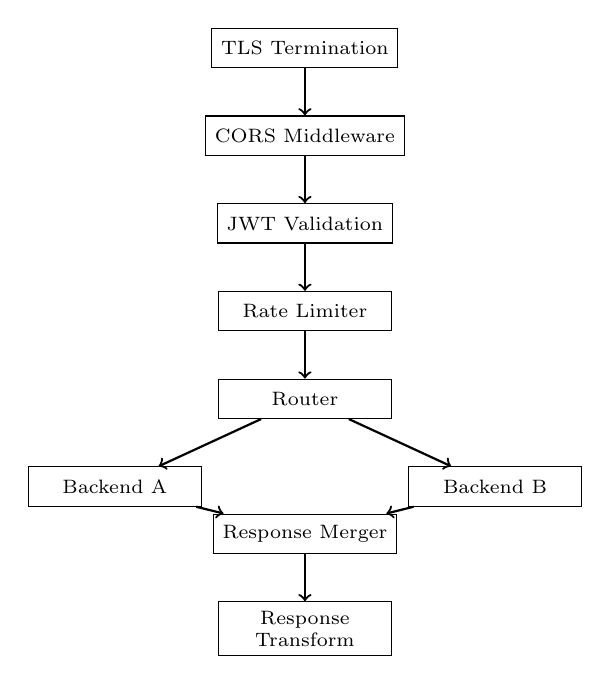
\begin{tikzpicture}[
    node distance=0.6cm,
    box/.style={rectangle, draw, minimum width=2.2cm, minimum height=0.5cm, align=center, font=\scriptsize},
    arrow/.style={->, thick}
]
\node[box] (ingress) {TLS Termination};
\node[box, below=of ingress] (cors) {CORS Middleware};
\node[box, below=of cors] (auth) {JWT Validation};
\node[box, below=of auth] (rate) {Rate Limiter};
\node[box, below=of rate] (route) {Router};
\node[box, below left=0.6cm and 0.2cm of route] (b1) {Backend A};
\node[box, below right=0.6cm and 0.2cm of route] (b2) {Backend B};
\node[box, below=1.2cm of route] (merge) {Response Merger};
\node[box, below=of merge] (transform) {Response\\Transform};

\draw[arrow] (ingress) -- (cors);
\draw[arrow] (cors) -- (auth);
\draw[arrow] (auth) -- (rate);
\draw[arrow] (rate) -- (route);
\draw[arrow] (route) -- (b1);
\draw[arrow] (route) -- (b2);
\draw[arrow] (b1) -- (merge);
\draw[arrow] (b2) -- (merge);
\draw[arrow] (merge) -- (transform);
\end{tikzpicture}
\caption{Gateway request processing pipeline.}
\label{fig:pipeline}
\end{figure}

Each request passes through a deterministic pipeline (Figure~\ref{fig:pipeline}): TLS termination, CORS enforcement, JWT validation, rate limiting, routing, backend fan-out, response merging, and output transformation. The pipeline is configured declaratively---no imperative middleware chains.

\subsection{Configuration Model}

The gateway configuration is a single JSON document:

\begin{lstlisting}[language=JSON]
{
  "version": 3,
  "timeout": "3s",
  "endpoints": [{
    "endpoint": "/v1/users/{id}",
    "method": "GET",
    "backend": [{
      "host": ["http://user-svc:8080"],
      "url_pattern": "/users/{id}",
      "mapping": {
        "email": "user_email"
      }
    }],
    "extra_config": {
      "auth/validator": {
        "alg": "RS256",
        "jwk_url": "https://hanzo.id/.well-known/jwks.json",
        "roles_key": "roles",
        "roles": ["admin", "user"]
      }
    }
  }]
}
\end{lstlisting}

This declarative model eliminates the need for gateway-specific code. New endpoints are added by editing the configuration and triggering a reload.

\section{Key Features}

\subsection{JWT Validation}

The gateway validates JWTs against Hanzo IAM's JWKS endpoint. Keys are cached in memory and refreshed every 15 minutes or on validation failure (indicating key rotation). Validation checks:

\begin{enumerate}
    \item Signature verification (RS256/ES256)
    \item Expiration and not-before claims
    \item Issuer matches \texttt{https://hanzo.id}
    \item Audience matches the service identifier
    \item Required roles present in the \texttt{roles} claim
\end{enumerate}

The \texttt{owner} claim is propagated to backends via the \texttt{X-Hanzo-Org} header, enabling downstream services to scope queries without re-parsing the JWT.

\subsection{Rate Limiting}

Rate limits are enforced using in-memory sliding window counters keyed by $(\text{tenant}, \text{endpoint})$. The algorithm divides time into fixed windows and interpolates the count from the current and previous window:

\begin{equation}
    \text{count} = c_{\text{prev}} \times (1 - t/w) + c_{\text{curr}}
\end{equation}

where $c_{\text{prev}}$ and $c_{\text{curr}}$ are the previous and current window counts, $t$ is elapsed time in the current window, and $w$ is the window duration.

Default limits are 1,000 requests per minute per tenant, configurable per endpoint. Rate limit headers (\texttt{X-Rate-Limit-Remaining}, \texttt{Retry-After}) are included in all responses.

\subsection{Circuit Breaker}

Each backend connection is protected by a circuit breaker with three states: closed (normal), open (failing), and half-open (probing). The breaker opens after 5 consecutive failures or when the error rate exceeds 50\% over a 10-second window. In the open state, requests receive an immediate 503 response. After 30 seconds, the breaker enters half-open and allows a single probe request.

\subsection{Backend Aggregation}

A single gateway endpoint can fan out to multiple backends and merge responses:

\begin{lstlisting}[language=JSON]
{
  "endpoint": "/v1/dashboard",
  "backend": [
    {"host": ["http://user-svc:8080"],
     "url_pattern": "/user/me"},
    {"host": ["http://billing-svc:8080"],
     "url_pattern": "/billing/summary"},
    {"host": ["http://usage-svc:8080"],
     "url_pattern": "/usage/current"}
  ],
  "extra_config": {
    "proxy": {"sequential": false}
  }
}
\end{lstlisting}

Parallel fan-out reduces latency to the maximum of backend latencies rather than the sum.

\section{Implementation}

The gateway is built on KrakenD Community Edition with custom Go plugins for Hanzo-specific functionality. The total codebase is approximately 8,000 lines of Go (plugins) plus the KrakenD core.

\paragraph{Zero-Downtime Reloads.} Configuration changes are applied via Kubernetes rolling restarts. The gateway starts accepting connections on the new configuration before draining the old instance, achieving zero-downtime configuration updates.

\paragraph{Observability.} Every request generates a Prometheus histogram observation keyed by endpoint, method, status code, and backend. Custom metrics track JWT validation latency, rate limit rejections, and circuit breaker state transitions.

\begin{table}[h]
\centering
\caption{Gateway overhead per request (ms).}
\label{tab:overhead}
\begin{tabular}{lrr}
\toprule
\textbf{Component} & \textbf{p50} & \textbf{p99} \\
\midrule
TLS + CORS & 0.2 & 0.5 \\
JWT validation & 0.3 & 0.8 \\
Rate limit check & 0.05 & 0.1 \\
Routing & 0.1 & 0.2 \\
Response merge & 0.15 & 0.4 \\
\midrule
\textbf{Total overhead} & \textbf{0.8} & \textbf{2.0} \\
\bottomrule
\end{tabular}
\end{table}

\section{Security}

\paragraph{TLS.} All external traffic is TLS~1.3 only. Internal traffic between gateway and backends uses mTLS with certificates issued by Hanzo's internal CA.

\paragraph{CORS.} Cross-Origin Resource Sharing is enforced at the gateway level with per-endpoint origin whitelists. Preflight responses are cached for 24 hours.

\paragraph{Request Validation.} Maximum request body size (10MB default), header count limits, and URL length limits prevent abuse. Malformed requests are rejected before reaching backends.

\paragraph{Secret Management.} Backend URLs, API keys, and JWKS URLs are resolved from Hanzo KMS at startup. No secrets appear in the configuration file.

\section{Conclusion}

Hanzo Gateway provides a stateless, high-performance API gateway that adds less than 2ms of overhead to the critical request path. The declarative configuration model enables rapid endpoint management without code changes, while the circuit breaker and rate limiting systems protect backend services from cascading failures. The stateless architecture enables simple horizontal scaling---adding capacity requires only deploying additional replicas.

\bibliographystyle{plain}
\begin{thebibliography}{10}

\bibitem{krakend2017}
KrakenD. Ultra performant API Gateway with middlewares. 2017.

\bibitem{nygard2007}
M. Nygard. Release It! Design and Deploy Production-Ready Software. Pragmatic Bookshelf, 2007.

\bibitem{jwt2015}
M. Jones et al. JSON Web Token (JWT). RFC 7519, 2015.

\bibitem{sliding2019}
K. Veeraraghavan et al. Sliding Window Rate Limiters. ACM SoCC, 2019.

\end{thebibliography}

\end{document}
